%!TEX TS-program = xelatex

\documentclass[]{cv-class}
\usepackage{afterpage}
\usepackage{hyperref}
\usepackage{color}
\usepackage{xcolor}
\hypersetup{
    colorlinks=true,
    linkcolor=blue
}
\addbibresource{bibliography.bib}
\RequirePackage{xcolor}
\usepackage[utf8]{inputenc}
\usepackage[english]{babel} 
\usepackage[usenames, dvipsnames]{color}

\begin{document}

\begin{aside}
\color{blue}
  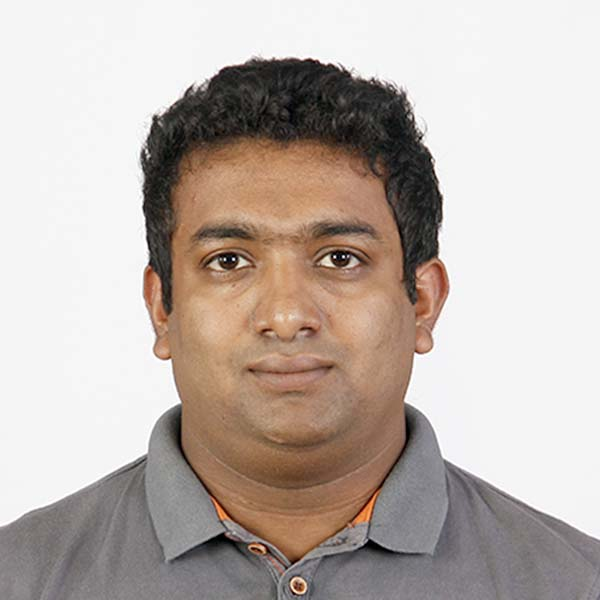
\includegraphics[scale=0.9]{img/photo.jpg}
    ~
  \header{Janitha}{Madushan}
      {Software Engineer}
   ~
  \section{ADDRESS}
    {\whitebodyfont No:04, "SunHill",\\
    Vajirapura,\\
    Nuwara-Eliya,\\
    Sri-Lanka.}
    ~
  \section{MOBILE}
    {\whitebodyfont +94 71 57 81 553\\
    +94 75 97 46 502}
    ~
  \section{MAILING}
    \underline{\href{mailto:janithasen@gmail.com}{{\whitebodyfont janithasen@gmail.com}}}
    ~
  \section{LANGAUGES}
  	{\whitebodyfont Sinhalese (Native)\\
    Engilsh}
    ~ 
  \section{NIC}
  	{\whitebodyfont 901540160V}
    ~
  \section{BIRTHDAY}
  	{\whitebodyfont June 02,1990}
    ~   
  \section{WEB}
  	\vspace{0.10cm}
    \underline{\href{https://www.linkedin.com/in/janithamadushan}{{\whitebodyfont Linkedin}}}
    \\
	\vspace{0.10cm}
    \underline{\href{https://stackoverflow.com/story/jmadushan}{{\whitebodyfont Stackoverflow}}}
	\\	
	\vspace{0.10cm}
    \underline{\href{https://github.com/janitham}{{\whitebodyfont Github}}}
    ~
  \section{OS PREFERENCES}
    \asidelist{{\whitebodyfont Windows}}
    {\includegraphics[scale=0.30]{img/star.png}
    \includegraphics[scale=0.30]{img/star.png}
    \includegraphics[scale=0.30]{img/star.png}
    \includegraphics[scale=0.30]{img/star.png}
    \includegraphics[scale=0.30]{img/star.png}}
    \asidelist{\whitebodyfont{Linux}}
    {\includegraphics[scale=0.30]{img/star.png}
    \includegraphics[scale=0.30]{img/star.png}
    \includegraphics[scale=0.30]{img/star.png}
    \includegraphics[scale=0.30]{img/star_empty.png}
    \includegraphics[scale=0.30]{img/star_empty.png}}
    ~
  \section{PROGRAMMING}
    \asidelist{{\whitebodyfont Java}}
    {\includegraphics[scale=0.30]{img/star.png}
    \includegraphics[scale=0.30]{img/star.png}
    \includegraphics[scale=0.30]{img/star.png}
    \includegraphics[scale=0.30]{img/star.png}
    \includegraphics[scale=0.30]{img/star_empty.png}}
    \asidelist{\whitebodyfont{C}}
    {\includegraphics[scale=0.30]{img/star.png}
    \includegraphics[scale=0.30]{img/star.png}
    \includegraphics[scale=0.30]{img/star.png}
    \includegraphics[scale=0.30]{img/star.png}
    \includegraphics[scale=0.30]{img/star_empty.png}}
    \asidelist{\whitebodyfont{Pyhon}}
    {\includegraphics[scale=0.30]{img/star.png}
    \includegraphics[scale=0.30]{img/star.png}
    \includegraphics[scale=0.30]{img/star.png}
    \includegraphics[scale=0.30]{img/star_empty.png}
    \includegraphics[scale=0.30]{img/star_empty.png}}
    \asidelist{\whitebodyfont{.NET}}
    {\includegraphics[scale=0.30]{img/star.png}
    \includegraphics[scale=0.30]{img/star.png}
    \includegraphics[scale=0.30]{img/star.png}
    \includegraphics[scale=0.30]{img/star_empty.png}
    \includegraphics[scale=0.30]{img/star_empty.png}}
    \asidelist{\whitebodyfont{PHP}}
    {\includegraphics[scale=0.30]{img/star.png}
    \includegraphics[scale=0.30]{img/star.png}
    \includegraphics[scale=0.30]{img/star.png}
    \includegraphics[scale=0.30]{img/star_empty.png}
    \includegraphics[scale=0.30]{img/star_empty.png}}
    ~
\end{aside}

\section{EXPERIENCE}
\begin{entrylist}
  \entry
    {Nov. 15 - Now}
    {Software Developer}
    {Cambio Software Engineering}
    {I am working in automation team which is a sub team of configuration management team, as a software developer. My responsibility is to automate manual tasks \& develop tools in continuous delivery, continuous integration and management tools. On that tasks, I developed various tools using various technologies. Mainly I developed tools using JAVA, Spring, Hibernate, AngularJs, maven-plugins(MOJO) and various technologies.}
\\
  \entry
    {Oct. 15 - Mar.16}
    {Internship}
    {IFS R\&D}
    {During my Internship I involved in two different projects, internal application and research project. In that period I exposed to ASP.NET, ORACLE 11G/12C, PLSQL, ORACLE-APEX, ANDROID and JAVA.}
\end{entrylist}

\section{EDUCATION}
\begin{entrylist}
  \entry
    {Aug. 11 - June 15}
    {Computer Engineering}
    {Faculty of Engineering, University of Peradeniya}
    {I followed Computer Engineering at Faculty of Engineering of University of Peradeniya, Sri-Lanka. I specified in Software Engineering.}
\end{entrylist}

\section{PROJECTS}
\begin{entrylist}
\entry
    {}
	{Snooper}    
    {Packaging(Installation Distribution) Data Management Tool}
{This is a sub-project of package-automation(Stacker) project. This application stores the packaging information. Snooper provides and Restful-API and GUI to do the necessary operations.\\Snooper architecture is based on micro-services-architecture. It is used micro-service architectures with Spring Cloud and Docker.\\\textbf{(Spring-cloud, Spring-boot, Hibernate, Ms-Sql, AngularJs, Java, Docker)}}
\\
\entry
    {}
	{Stacker}    
    {Packaging Automation Tool(Continuous Delivery, Team CI)}
    {Stacker is continuous delivery automation tool. This works on fully mavenized environment. Stacker can be used as an JAVA application or as a maven-plugin, it generates multi-module pom structure configured with different maven plugins(Two 			different frameworks are used in the product, packaging is done in different orders), using matadata(An artifact is released to nexus). Finally the package can be generated using the pom structure which is based on the baseline. \\This stacker is recently using as a maven plugin which is configured in a Jenkins job, the job has also integrated with JIRA(using JIRA \& Jenkins plugins). Now, the package requester can create the package him self. \\Stacker has also configured as a pipeline in the Jenkis-job. Also a maven plugin is used to update package information management tool(Snooper) using it's Restful-APIs'.\\\textbf{(Java, Maven-plugins, Jenkins, Jenkins-pipelines, Nexus, JIRA)}}
\end{entrylist}


\newpage
\begin{aside}
\end{aside}

\begin{entrylist}
	\entry
    {}
	{ART}    
    {Archetypes Replacement Tool(Continuous Delivery)}
{Previous days we had Maven-based Archetypes to generate packaging pom structures to create specific distributions. ART tool is a web based solution to create the packaging structures. Any user can login using AD and admins are only allowed to maintain configurations.\\\textbf{(JAVA, Spring, AngularJs, Spring-Security, Hibernate, JBoss, SOA)}}
	\\
	\entry
    {}
    {Microphone Alternator of Android}
    {Computer Engineering Project}
    {This system mainly has clients and main server application. The client requests to connect with the server application using multi-casting. Subsequently, the client gets the access token to connect to server then the particular client can start uni-casting the sound stream (thorough Android smart-phones). The server application plays the sound stream. \\\textbf{(Android, Java, UDP Socket Programming, multi-casting, uni-casting)}}
    \\
	\entry
    {}
    {Device Dependent CAPTHCHA System}
    {Final Year Project}
    {CAPTCHA system that provides suitable CAPTCHAs for suitable devices by  detecting  the  device,  then  provides  the  CAPTCHAs  as  their functionalities and usability.}
	\\
  \entry
    {}
    {IFS Rest Data service}
    {Internship Project}
    {Research on exposing database as  RESTful  services. Demonstrated  using  MS  excel  office  application.\\\textbf{(ORACLE 12/C, ORACLE-APEX, OFFICE-APPS, PL-SQL)}}
	\\
  \entry
    {}
    {IFS Day-Care Application}
    {Internship Project}
    {Web  based  application  used  by  IFS  employees  to  reserve  the  day-care facility at IFS. \\\textbf{(ASP.NET, PLSQL, Oracle 11g database, Android, Java)}}
	\\  
  \entry
    {}
    {Multi-User Chat Room}
    {Computer Engineering Project}
    {Particular number of clients can be connected with the server. If any 
	client  sends  a  message, subsequently  the  massage  will be broadcasted to the other clients. 
	\\\textbf{(C, Socket Programming, Multi-Threading)}}
	\\
  \entry
    {}
    {Tag Cloud}
    {Computer Engineering Project}
    {Get most frequent words from multiple HTML files which are in 
	multiple directories and creates a tag cloud out of those words using a 
	SVG. \\\textbf{(C, Unix Shell Scripting, Multi-Processing )}}
\end{entrylist}

\begin{entrylist}
  \entry
    {}
    {}
    {}
    {References upon Request}
  \entry
    {}
    {}
    {}
    {I do here by certify that above particulars are true and correct. If you are pleased to consider me 
	suitable for your company and select me as an employee, it will be my earnest endeavor to discharge 
	the duties entrusted to me, to the best of my ability and rise to your expectations.}
\end{entrylist}

\begin{flushright}
\emph{Janitha Madushan}
\end{flushright}
\begin{flushright}
\emph{\today}
\end{flushright}

\end{document}